
%% bare_conf.tex
%% V1.3
%% 2007/01/11
%% by Michael Shell
%% See:
%% http://www.michaelshell.org/
%% for current contact information.
%%
%% This is a skeleton file demonstrating the use of IEEEtran.cls
%% (requires IEEEtran.cls version 1.7 or later) with an IEEE conference paper.
%%
%% Support sites:
%% http://www.michaelshell.org/tex/ieeetran/
%% http://www.ctan.org/tex-archive/macros/latex/contrib/IEEEtran/
%% and
%% http://www.ieee.org/

%%*************************************************************************
%% Legal Notice:
%% This code is offered as-is without any warranty either expressed or
%% implied; without even the implied warranty of MERCHANTABILITY or
%% FITNESS FOR A PARTICULAR PURPOSE!
%% User assumes all risk.
%% In no event shall IEEE or any contributor to this code be liable for
%% any damages or losses, including, but not limited to, incidental,
%% consequential, or any other damages, resulting from the use or misuse
%% of any information contained here.
%%
%% All comments are the opinions of their respective authors and are not
%% necessarily endorsed by the IEEE.
%%
%% This work is distributed under the LaTeX Project Public License (LPPL)
%% ( http://www.latex-project.org/ ) version 1.3, and may be freely used,
%% distributed and modified. A copy of the LPPL, version 1.3, is included
%% in the base LaTeX documentation of all distributions of LaTeX released
%% 2003/12/01 or later.
%% Retain all contribution notices and credits.
%% ** Modified files should be clearly indicated as such, including  **
%% ** renaming them and changing author support contact information. **
%%
%% File list of work: IEEEtran.cls, IEEEtran_HOWTO.pdf, bare_adv.tex,
%%                    bare_conf.tex, bare_jrnl.tex, bare_jrnl_compsoc.tex
%%*************************************************************************

% *** Authors should verify (and, if needed, correct) their LaTeX system  ***
% *** with the testflow diagnostic prior to trusting their LaTeX platform ***
% *** with production work. IEEE's font choices can trigger bugs that do  ***
% *** not appear when using other class files.                            ***
% The testflow support page is at:
% http://www.michaelshell.org/tex/testflow/



% Note that the a4paper option is mainly intended so that authors in
% countries using A4 can easily print to A4 and see how their papers will
% look in print - the typesetting of the document will not typically be
% affected with changes in paper size (but the bottom and side margins will).
% Use the testflow package mentioned above to verify correct handling of
% both paper sizes by the user's LaTeX system.
%
% Also note that the "draftcls" or "draftclsnofoot", not "draft", option
% should be used if it is desired that the figures are to be displayed in
% draft mode.
%
\documentclass[conference]{IEEEtran}
% Add the compsoc option for Computer Society conferences.
%
% If IEEEtran.cls has not been installed into the LaTeX system files,
% manually specify the path to it like:
% \documentclass[conference]{../sty/IEEEtran}





% Some very useful LaTeX packages include:
% (uncomment the ones you want to load)


% *** MISC UTILITY PACKAGES ***
%
%\usepackage{ifpdf}
% Heiko Oberdiek's ifpdf.sty is very useful if you need conditional
% compilation based on whether the output is pdf or dvi.
% usage:
% \ifpdf
%   % pdf code
% \else
%   % dvi code
% \fi
% The latest version of ifpdf.sty can be obtained from:
% http://www.ctan.org/tex-archive/macros/latex/contrib/oberdiek/
% Also, note that IEEEtran.cls V1.7 and later provides a builtin
% \ifCLASSINFOpdf conditional that works the same way.
% When switching from latex to pdflatex and vice-versa, the compiler may
% have to be run twice to clear warning/error messages.






% *** CITATION PACKAGES ***
%
%\usepackage{cite}
% cite.sty was written by Donald Arseneau
% V1.6 and later of IEEEtran pre-defines the format of the cite.sty package
% \cite{} output to follow that of IEEE. Loading the cite package will
% result in citation numbers being automatically sorted and properly
% "compressed/ranged". e.g., [1], [9], [2], [7], [5], [6] without using
% cite.sty will become [1], [2], [5]--[7], [9] using cite.sty. cite.sty's
% \cite will automatically add leading space, if needed. Use cite.sty's
% noadjust option (cite.sty V3.8 and later) if you want to turn this off.
% cite.sty is already installed on most LaTeX systems. Be sure and use
% version 4.0 (2003-05-27) and later if using hyperref.sty. cite.sty does
% not currently provide for hyperlinked citations.
% The latest version can be obtained at:
% http://www.ctan.org/tex-archive/macros/latex/contrib/cite/
% The documentation is contained in the cite.sty file itself.





%\usepackage{graphicx}
% *** GRAPHICS RELATED PACKAGES ***
%
\ifCLASSINFOpdf
   \usepackage[pdftex]{graphicx}
  % declare the path(s) where your graphic files are
  % \graphicspath{{../pdf/}{../jpeg/}}
  % and their extensions so you won't have to specify these with
  % every instance of \includegraphics
  % \DeclareGraphicsExtensions{.pdf,.jpeg,.png}
\else
  % or other class option (dvipsone, dvipdf, if not using dvips). graphicx
  % will default to the driver specified in the system graphics.cfg if no
  % driver is specified.
   \usepackage[dvips]{graphicx}
  % declare the path(s) where your graphic files are
  % \graphicspath{{../eps/}}
  % and their extensions so you won't have to specify these with
  % every instance of \includegraphics
  % \DeclareGraphicsExtensions{.eps}
\fi
% graphicx was written by David Carlisle and Sebastian Rahtz. It is
% required if you want graphics, photos, etc. graphicx.sty is already
% installed on most LaTeX systems. The latest version and documentation can
% be obtained at:
% http://www.ctan.org/tex-archive/macros/latex/required/graphics/
% Another good source of documentation is "Using Imported Graphics in
% LaTeX2e" by Keith Reckdahl which can be found as epslatex.ps or
% epslatex.pdf at: http://www.ctan.org/tex-archive/info/
%
% latex, and pdflatex in dvi mode, support graphics in encapsulated
% postscript (.eps) format. pdflatex in pdf mode supports graphics
% in .pdf, .jpeg, .png and .mps (metapost) formats. Users should ensure
% that all non-photo figures use a vector format (.eps, .pdf, .mps) and
% not a bitmapped formats (.jpeg, .png). IEEE frowns on bitmapped formats
% which can result in "jaggedy"/blurry rendering of lines and letters as
% well as large increases in file sizes.
%
% You can find documentation about the pdfTeX application at:
% http://www.tug.org/applications/pdftex





% *** MATH PACKAGES ***
%
%\usepackage[cmex10]{amsmath}
% A popular package from the American Mathematical Society that provides
% many useful and powerful commands for dealing with mathematics. If using
% it, be sure to load this package with the cmex10 option to ensure that
% only type 1 fonts will utilized at all point sizes. Without this option,
% it is possible that some math symbols, particularly those within
% footnotes, will be rendered in bitmap form which will result in a
% document that can not be IEEE Xplore compliant!
%
% Also, note that the amsmath package sets \interdisplaylinepenalty to 10000
% thus preventing page breaks from occurring within multiline equations. Use:
%\interdisplaylinepenalty=2500
% after loading amsmath to restore such page breaks as IEEEtran.cls normally
% does. amsmath.sty is already installed on most LaTeX systems. The latest
% version and documentation can be obtained at:
% http://www.ctan.org/tex-archive/macros/latex/required/amslatex/math/





% *** SPECIALIZED LIST PACKAGES ***
%
%\usepackage{algorithmic}
% algorithmic.sty was written by Peter Williams and Rogerio Brito.
% This package provides an algorithmic environment fo describing algorithms.
% You can use the algorithmic environment in-text or within a figure
% environment to provide for a floating algorithm. Do NOT use the algorithm
% floating environment provided by algorithm.sty (by the same authors) or
% algorithm2e.sty (by Christophe Fiorio) as IEEE does not use dedicated
% algorithm float types and packages that provide these will not provide
% correct IEEE style captions. The latest version and documentation of
% algorithmic.sty can be obtained at:
% http://www.ctan.org/tex-archive/macros/latex/contrib/algorithms/
% There is also a support site at:
% http://algorithms.berlios.de/index.html
% Also of interest may be the (relatively newer and more customizable)
% algorithmicx.sty package by Szasz Janos:
% http://www.ctan.org/tex-archive/macros/latex/contrib/algorithmicx/




% *** ALIGNMENT PACKAGES ***
%
%\usepackage{array}
% Frank Mittelbach's and David Carlisle's array.sty patches and improves
% the standard LaTeX2e array and tabular environments to provide better
% appearance and additional user controls. As the default LaTeX2e table
% generation code is lacking to the point of almost being broken with
% respect to the quality of the end results, all users are strongly
% advised to use an enhanced (at the very least that provided by array.sty)
% set of table tools. array.sty is already installed on most systems. The
% latest version and documentation can be obtained at:
% http://www.ctan.org/tex-archive/macros/latex/required/tools/


%\usepackage{mdwmath}
%\usepackage{mdwtab}
% Also highly recommended is Mark Wooding's extremely powerful MDW tools,
% especially mdwmath.sty and mdwtab.sty which are used to format equations
% and tables, respectively. The MDWtools set is already installed on most
% LaTeX systems. The lastest version and documentation is available at:
% http://www.ctan.org/tex-archive/macros/latex/contrib/mdwtools/


% IEEEtran contains the IEEEeqnarray family of commands that can be used to
% generate multiline equations as well as matrices, tables, etc., of high
% quality.


%\usepackage{eqparbox}
% Also of notable interest is Scott Pakin's eqparbox package for creating
% (automatically sized) equal width boxes - aka "natural width parboxes".
% Available at:
% http://www.ctan.org/tex-archive/macros/latex/contrib/eqparbox/





% *** SUBFIGURE PACKAGES ***
%\usepackage[tight,footnotesize]{subfigure}
% subfigure.sty was written by Steven Douglas Cochran. This package makes it
% easy to put subfigures in your figures. e.g., "Figure 1a and 1b". For IEEE
% work, it is a good idea to load it with the tight package option to reduce
% the amount of white space around the subfigures. subfigure.sty is already
% installed on most LaTeX systems. The latest version and documentation can
% be obtained at:
% http://www.ctan.org/tex-archive/obsolete/macros/latex/contrib/subfigure/
% subfigure.sty has been superceeded by subfig.sty.



%\usepackage[caption=false]{caption}
%\usepackage[font=footnotesize][caption=false]{subfig}
% subfig.sty, also written by Steven Douglas Cochran, is the modern
% replacement for subfigure.sty. However, subfig.sty requires and
% automatically loads Axel Sommerfeldt's caption.sty which will override
% IEEEtran.cls handling of captions and this will result in nonIEEE style
% figure/table captions. To prevent this problem, be sure and preload
% caption.sty with its "caption=false" package option. This is will preserve
% IEEEtran.cls handing of captions. Version 1.3 (2005/06/28) and later
% (recommended due to many improvements over 1.2) of subfig.sty supports
% the caption=false option directly:
\usepackage[caption=false,font=footnotesize]{subfig}
%\usepackage{subfigure}
%\usepackage{caption}

%
% The latest version and documentation can be obtained at:
% http://www.ctan.org/tex-archive/macros/latex/contrib/subfig/
% The latest version and documentation of caption.sty can be obtained at:
% http://www.ctan.org/tex-archive/macros/latex/contrib/caption/




% *** FLOAT PACKAGES ***
%
%\usepackage{fixltx2e}
% fixltx2e, the successor to the earlier fix2col.sty, was written by
% Frank Mittelbach and David Carlisle. This package corrects a few problems
% in the LaTeX2e kernel, the most notable of which is that in current
% LaTeX2e releases, the ordering of single and double column floats is not
% guaranteed to be preserved. Thus, an unpatched LaTeX2e can allow a
% single column figure to be placed prior to an earlier double column
% figure. The latest version and documentation can be found at:
% http://www.ctan.org/tex-archive/macros/latex/base/



%\usepackage{stfloats}
% stfloats.sty was written by Sigitas Tolusis. This package gives LaTeX2e
% the ability to do double column floats at the bottom of the page as well
% as the top. (e.g., "\begin{figure*}[!b]" is not normally possible in
% LaTeX2e). It also provides a command:
%\fnbelowfloat
% to enable the placement of footnotes below bottom floats (the standard
% LaTeX2e kernel puts them above bottom floats). This is an invasive package
% which rewrites many portions of the LaTeX2e float routines. It may not work
% with other packages that modify the LaTeX2e float routines. The latest
% version and documentation can be obtained at:
% http://www.ctan.org/tex-archive/macros/latex/contrib/sttools/
% Documentation is contained in the stfloats.sty comments as well as in the
% presfull.pdf file. Do not use the stfloats baselinefloat ability as IEEE
% does not allow \baselineskip to stretch. Authors submitting work to the
% IEEE should note that IEEE rarely uses double column equations and
% that authors should try to avoid such use. Do not be tempted to use the
% cuted.sty or midfloat.sty packages (also by Sigitas Tolusis) as IEEE does
% not format its papers in such ways.





% *** PDF, URL AND HYPERLINK PACKAGES ***
%
%\usepackage{url}
% url.sty was written by Donald Arseneau. It provides better support for
% handling and breaking URLs. url.sty is already installed on most LaTeX
% systems. The latest version can be obtained at:
% http://www.ctan.org/tex-archive/macros/latex/contrib/misc/
% Read the url.sty source comments for usage information. Basically,
% \url{my_url_here}.





% *** Do not adjust lengths that control margins, column widths, etc. ***
% *** Do not use packages that alter fonts (such as pslatex).         ***
% There should be no need to do such things with IEEEtran.cls V1.6 and later.
% (Unless specifically asked to do so by the journal or conference you plan
% to submit to, of course. )


% correct bad hyphenation here
\hyphenation{op-tical net-works semi-conduc-tor}


\begin{document}
%
% paper title
% can use linebreaks \\ within to get better formatting as desired
\title{Information Diffusion on Twitter: everyone has its chance, but all chances are not equal}


% author names and affiliations
% use a multiple column layout for up to three different
% affiliations
\author{\IEEEauthorblockN{Cazabet Remy}
\IEEEauthorblockA{National Institute of Informatics\\
Tokyo, Japan\\
remy.cazabet@gmail.com}

\and

\IEEEauthorblockN{Nargis Pervin}
\IEEEauthorblockA{National University of Singapore\\
Singapore, Singapore\\
nargisp@comp.nus.edu.sg}

\and

\IEEEauthorblockN{Fujio Toriumi}
\IEEEauthorblockA{The university of Tokyo\\
Tokyo, Japan\\
tori@sys.t.u-tokyo.ac.jp}

\and

\IEEEauthorblockN{Hideaki Takeda}
\IEEEauthorblockA{National Institute of Informatics\\
Tokyo, Japan\\
takeda@nii.ac.jp}
}

% conference papers do not typically use \thanks and this command
% is locked out in conference mode. If really needed, such as for
% the acknowledgment of grants, issue a \IEEEoverridecommandlockouts
% after \documentclass

% for over three affiliations, or if they all won't fit within the width
% of the page, use this alternative format:
%
%\author{\IEEEauthorblockN{Michael Shell\IEEEauthorrefmark{1},
%Homer Simpson\IEEEauthorrefmark{2},
%James Kirk\IEEEauthorrefmark{3},
%Montgomery Scott\IEEEauthorrefmark{3} and
%Eldon Tyrell\IEEEauthorrefmark{4}}
%\IEEEauthorblockA{\IEEEauthorrefmark{1}School of Electrical and Computer Engineering\\
%Georgia Institute of Technology,
%Atlanta, Georgia 30332--0250\\ Email: see http://www.michaelshell.org/contact.html}
%\IEEEauthorblockA{\IEEEauthorrefmark{2}Twentieth Century Fox, Springfield, USA\\
%Email: homer@thesimpsons.com}
%\IEEEauthorblockA{\IEEEauthorrefmark{3}Starfleet Academy, San Francisco, California 96678-2391\\
%Telephone: (800) 555--1212, Fax: (888) 555--1212}
%\IEEEauthorblockA{\IEEEauthorrefmark{4}Tyrell Inc., 123 Replicant Street, Los Angeles, California 90210--4321}}




% use for special paper notices
%\IEEEspecialpapernotice{(Invited Paper)}




% make the title area
\maketitle


\begin{abstract}
%\boldmath
Twitter is a web 2.0 social network which attracted much attention recently for its usage as an alternative media for information diffusion. From the recent events in arab countries, to natural disaster such as earthquakes or tsunamis, Twitter has proven to be a credible alternative to traditional means of information diffusion. Relatively few works have been done on this question of information diffusion, and in particular on the relative importance of different kind of users on this question. In this paper, we show that all users are not equal on the aspect of information diffusion. By investigating thoroughly the retweet chain lengths of users on a large dataset, we found that the number of followers of users plays an important role in their capacity to propagate information. From our observations we propose a very simple model, which is accurate enough to generate realistic length of retweet chains on the network. We consequently show, by studying a Twitter dataset centered on the Japanese Earthquake and Tsunami in March 2011, that such a crisis impact greatly the propagation of information. Finally, we use our results to discuss on the means of improving information diffusion to reach targeted users.


\end{abstract}
% IEEEtran.cls defaults to using nonbold math in the Abstract.
% This preserves the distinction between vectors and scalars. However,
% if the conference you are submitting to favors bold math in the abstract,
% then you can use LaTeX's standard command \boldmath at the very start
% of the abstract to achieve this. Many IEEE journals/conferences frown on
% math in the abstract anyway.

% no keywords




% For peer review papers, you can put extra information on the cover
% page as needed:
% \ifCLASSOPTIONpeerreview
% \begin{center} \bfseries EDICS Category: 3-BBND \end{center}
% \fi
%
% For peerreview papers, this IEEEtran command inserts a page break and
% creates the second title. It will be ignored for other modes.
\IEEEpeerreviewmaketitle



\section{Introduction}
% no \IEEEPARstart
Web 2.0 social networks platforms, such as Facebook, Twitter, Google Plus or Flickr, have attracted lot of attention in the recent years. As more and more users join them, new usages develop, and their role in society increase. Twitter is one of the most influential platform, as highlighted by recent events. Two examples are now especially famous: first, the key role played by Twitter during the so-called arab spring (see, for example, \cite{howard2011opening}), during which insurgents used it as a major way of organization and as an information source. Secondly, in an unrelated topic, during the 2011 earthquake and tsunami in Japan, during which users relayed information ranging from tsunami alert to rescue request, or more simply shared local information.

One key feature of Twitter, which makes it maybe the most efficient web 2.0 social network platform to share information in time of crisis, is that it is particularly suited for information diffusion. Unlike other platforms, there is no reciprocity needed in the relations, and therefore the most influential users can gather tens of thousands of so called followers, people who register to be informed of their publications. On the opposite side, as in others small world networks, most users have very few relations, ensuring a more convincing power law distribution of in-degree than, for instance, Facebook. The consequence is that different users can play very different roles in the network, in particular in terms of information diffusion.

In some previous works that we will present in the next section, authors have investigated the factors that could influence the success of the diffusion of a piece of information. Most works done to predict the success of tweets based on their content have resulted in relatively poor results. If their is for sure a relation between the content of a tweet and it's probability to be retweeted, it seems nearly impossible to predict the success of a future tweet based on its content, or to derive a model which could generate realistic tweet diffusion based on what is said on the network.

More successes have been achieved by relying on the properties of the network itself, and in particular the properties of the user. The relation between the number of followers of a user (to which we will refer further as its in-degree) and the average length of its tweets has been shown several time.

The goal of this paper was to push further the study of this relation, which is, until now, the more reliable way of predicting the success of a tweet.

Our paper is organized as follows: after reviewing briefly related works in the next section, we will present the experiments we have conduced in order to describe more precisely the role of the number of followers in the probability to produce seminal tweets. We will then use these findings to propose a simple model, which allows us to generate, starting from the sequence of unique tweets posted by users in the network, chains of randomly generated lengths following the proposed model. We then check that the generated retweet chain length match real data, not only on the aggregated level, but also on the aspect of the relative influence of most popular and less popular users in the generation of long chains of retweet.
We will continue by showing that these retweeting behaviors can be strongly disrupted by an event such as a large earthquake.
Finally, in the last section, we will discuss how our findings can help to understand how it could be possible to optimize the probability of sharing a given information on the network.


\section{Related works}
The question of who are the key influential users, and why, has already attracted a lot of attention. One of the most influential work made on this topic is presented in Bakshy et al.  \cite{bakshy2011everyone}. The authors, after observing that the distribution of size of retweet chains were roughly following a power law, were interested in understanding which factors could explain the success of popular tweets. They found a correlation between the number of followers and the probability of producing a widely shared tweet. They also found, by asking people to classify tweets' content, that tweets with content classified as ``interesting" were more likely to spread. However, one important finding was that predicting which particular content or which particular user might produce a widely propagated tweet was mostly unreliable. They concluded that, if one wants to optimize the diffusion of a particular information, one must use a large number of sources users, relying on average effects.

In Suh et al. \cite{suh2010want}, several factors that could be correlated to the retweet success of tweets have been investigated. First, the authors have studied the correlation between the content of the tweet and its number of retweets. However, considering either the hashtags included in the tweets or the URLs did not show any convincing correlation. It is therefore likely that predicting the number of retweets  based on the content of the message would be very difficult, as such success can be highly influenced by a large number of factors, and in particular factors external to Twitter. The same tweet, for instance about the Fukushima power plant, published just before or just after the 2011 earthquake might result in very different spreading. In a second attempt, the authors studied how the properties of the tweet's author might impact the diffusion of his tweets. They found that the past number of published tweets had barely any impact.
On the contrary, they found a very strong and regular correlation between the number of followers of a user and the average number of retweets of their tweets.
They found that two other factors, the age of the tweeter account and the number of followees, had some kind of correlation with the average retweet count. However, these relations are not linear nor monotonic. Furthermore, one can note that both of them are not independent with the number of followers: the number of followers tend to increase with the age of the account, and users with more followees tend to have, in average, more followers, as it has been observed, for example, in Krishnamurthy et al. \cite{krishnamurthy2008few}.


Kwak et al. \cite{kwak2010twitter} have also investigated the relation between the number of followers of tweets' authors and their retweets. In their case, they studied more particularly the number of retweets made by users who were not direct followers of the original posters. Interestingly, they argue that users with less than 1000 followers tend to have the same average number of retweets. However, they do not display only the average retweet count, along with the median. And this median tends to increase with the number of followers. Therefore, we can assume that even though the average number of retweet do not change, the distribution of the retweet count of all tweets by the user changes with the number of followers.

Some other works have studied the influence of users, in particular Cha et al. \cite{cha2010measuring}, who found that users with high in-degrees are usually influential in term of new information, but some of them are not influential in term of retweeting. They also investigate the relation between influential users and different topics.



%\hfill mds

%\hfill January 11, 2007

\section{Dataset description}
\textbf{Tweet Data:} We used a Twitter dataset collected during the great Tohoku earthquake in Japan in March 2011 and described thoroughly in \cite{toriumi2013information}. The dataset covers a period of 20 days (from $5^{th}$ March, 2011 to $24^{th}$ March, 2011), and consists of 362,435,649 tweets posted by 2,711,473 users in Japan. This dataset is remarkable by its completeness: the authors have checked that 80\% to 90\% of all published tweets by these users were present in this dataset.

Fig.~\ref{fig:retweetdist} shows the normalized retweet count for 20 days of period. The first two major peaks represent the two big earthquakes on $11^{th}$ and $12^{th}$ March. After the disaster, retweet count progressively returns to its normal average values. \\



\noindent\textbf{Follower Network Data:} In Twitter, follower network depicts the social relationship among the users. Follower information has been collected by crawling Twitter API in May, 2013 for the active users who have been mentioned more than 20 times in the dataset.
Follower network dataset consists of 300,104 users and 73,446,260 relationships information. Degree distribution has been shown in Fig.~\ref{fig:followernet} by plotting cumulative fraction of users against the number of followers/followees of user.

We can note that this follower network is not complete, and collected after the events. However, in this work, we are not interested in the particular follower/followees relationships, but simply on the number of followers of each user, which is probably less sensitive. Nevertheless, we did not take simply the number of followers of the users from Twitter, bust instead counted how many followers in our dataset were following each particular user, to increase accuracy. For example, some users are very popular outside of Japan, and therefore have a large total number of followers, but are not followed by many of our selected users.

\begin{figure}[h]
    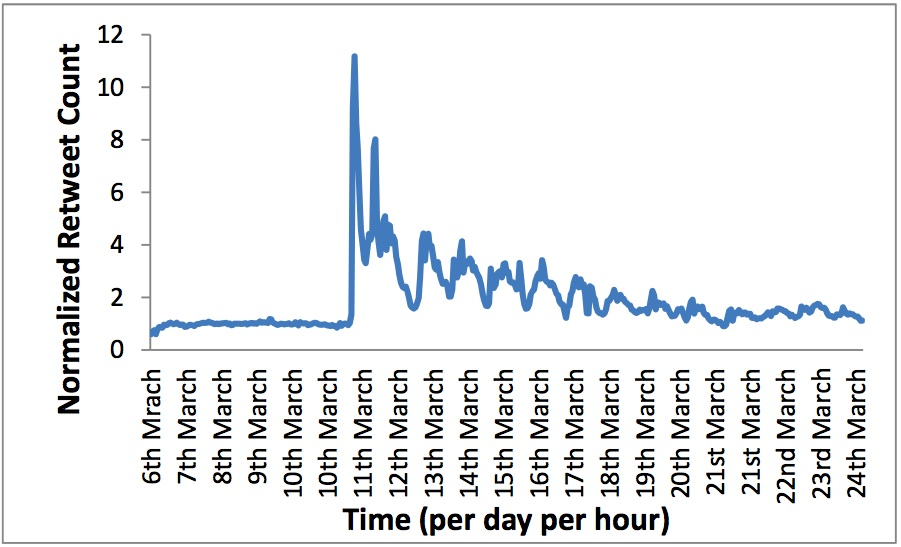
\includegraphics[width=0.5\textwidth]{data/retweetCount.jpg}
    \caption{Tweet Distribution over days (Normalized)}
    \label{fig:retweetdist}
\end{figure}


\begin{figure}[h]
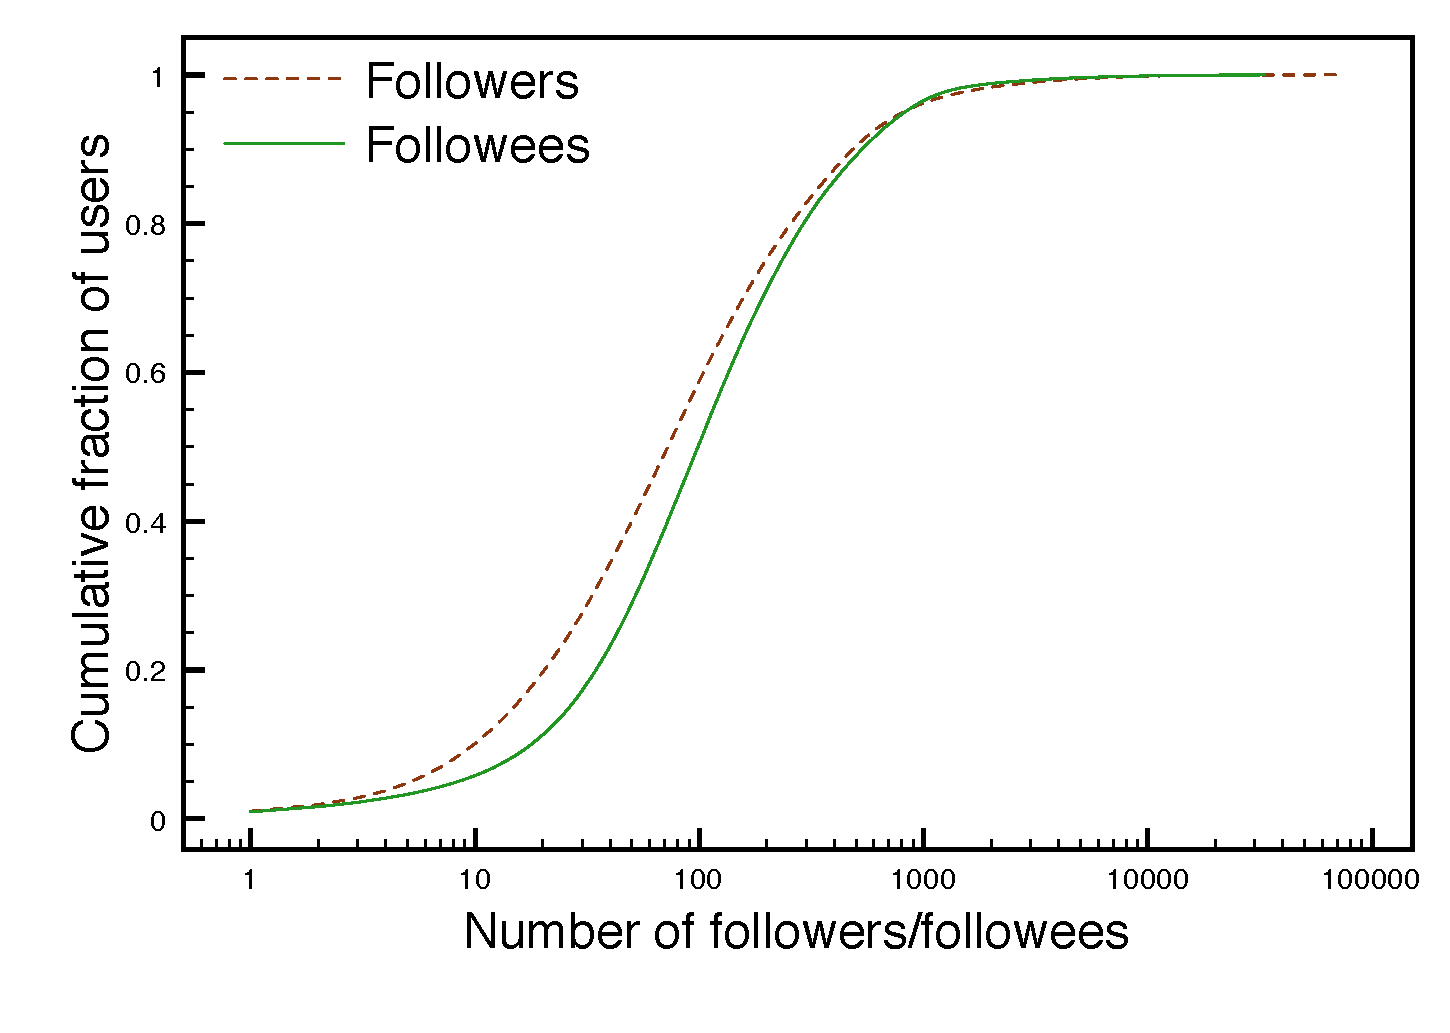
\includegraphics[width=0.5\textwidth]{data/degreesDistribution.eps}
\caption{Cumulative fraction of users by degree}

    \label{fig:followernet}
\end{figure}



\section{From observations to a simple model}

In the first part of this section, we will present some findings on the role played by the number of followers of a user in the propagation of its tweets. In the second part, we will validate that these findings are reasonably accurate by using them as base in a model for the generation of tweets diffusion.

\subsubsection{Retweet Chain Length distribution}


  \begin{figure}[h]
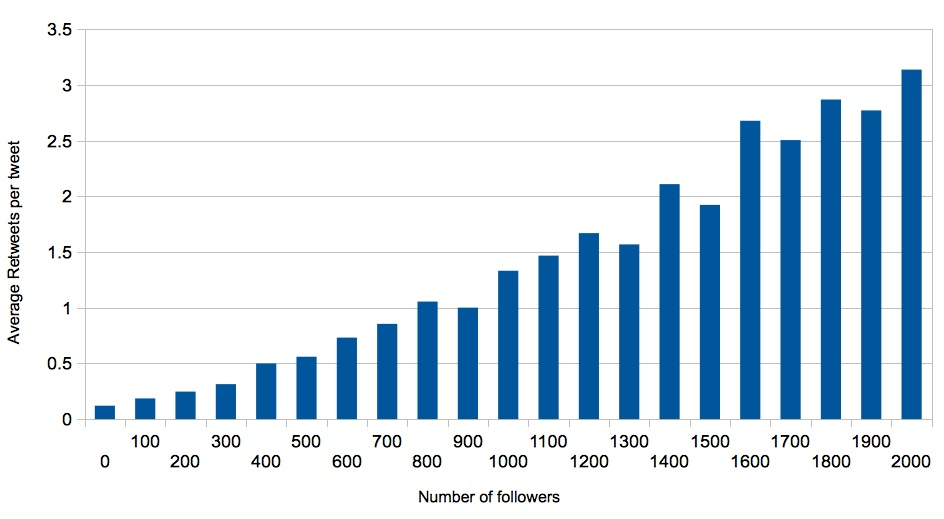
\includegraphics[width=0.5\textwidth]{data/averageRT.jpg}
\caption{Average number of retweets per tweet vs. the number of followers}

    \label{fig:averageRT}
\end{figure}

We first began to check, on our dataset, the correlation between the number of followers of a user and the average length of the retweet chains of the tweets he posts. This relation has already been discussed in other papers and have been validated on our dataset. We observed the same correlation as depicted in fig. \ref{fig:averageRT}.
Most works use a dataset collected by randomly choosing a relatively small portion of the tweets over a large number of users for long period of time. On the contrary, our dataset is more close to completeness, for a shorter period and with less users. To identify tweets belonging to the retweet chains, we first recognize all original tweets not containing the ``RT $@$" mention. In the second step, for each of these original tweets we counted all tweets of the form ``RT $@$" in which the section which appears at the right of the last RT mention is identical to the original tweet. This process might have some flaw as some retweets might not be formatted in the exact pattern that we are searching for (as identified by Boyd et al.\cite{boyd2010tweet}), but as the retweet functionality have been now implemented in most Twitter clients including the official one, a higher percentage of retweets are correctly formatted. Furthermore, the Japanese language needs far less characters than English on average for the same content, so it is probably less common to modify the original tweet for concision reasons.
%We observed the same correlation, as shown in fig. \ref{fig:averageRT}.

The corrleation in Fig. 3 is found on average retweet chain length. However, it is obvious that there is a great disparity in the length of retweet chains. Taking the average will loose the insight of the distribution of  retweet chain length. Moreover, it has been shown in \cite{bakshy2011everyone} that the overall distribution of retweet chain length follows a power law. As a consequence, computing an average value is mostly meaningless. Therefore, we searched to characterize the relation between followers and information diffusion, not through the mean diffusion, but through the evolution of the parameters of the power law representing this distribution.

In this paper, we observe several time the power law nature of some distributions. As it has been thoroughly discussed by Clauset et al. \cite{clauset2009power}, with the recent growth in interest for power law distribution some works claim to find power law distributions where they are not actually the best model for the observed distribution due to lack of rigor in the evaluation. To mitigate this issue in this paper we use maximum-likelihood to fit the curve instead of least-squares fitting. Further, using a goodness of fit test based on Kolmogorov-Smirnov statistic we checked whether power-law is in fact a good fit. Finally, we verify that a log-normal distribution is not an obvious better descriptor, as it is sometime the case. The power law nature of these distributions are not claimed as result of our work, but are used to represent the distribution and its evolution in convenient way. Statistically, the power law distribution is a very good approximation of the distribution. It could probably be possible to improve the accuracy by finely tuning a cut-off for it. But this cut-off will most likely depend on the size of the particular network, while we were more interested in a general relation between the in-degree of users and their probability to generate retweet chains of a given size.

\subsection{Influence of the number of followers}
We have validated (fig.~\ref{fig:averageRT}) that the number of followers of a user has an influence on the average retweet chains of tweets. Therefore, we know that they do not have the same probability distribution of being retweeted. In this section, we study how this distribution change with the number of followers.
To do so, we computed the distribution on the whole network, but only for users of a given number of followers. We restricted our analysis to the first five days of our dataset, from 5 to 9 of March, 2011 -days preceding the earthquake- as we thought that users might change their behaviors  after this event. Note that we kept one day, the 10 of March, in order to check that our finding were also valid on this day.

In order to have enough data for statistically significant results, in particular for users with large number of followers ($FC$) who are less common, we compute the distribution for all possible $i$  with all users $u$ such as $FC(u)=i, i*5 < FC(u) < (i+1)*5,i*10 < FC(u) < (i+1)*10, i*50 < FC(u) < (i+1)*50, i*100 <FC(u)*100, i*500 <FC(u)*500$ and $i*1000 <FC(u)*1000$.
Then, for each of these results, if we have a minimum of 10,000 chains with a strength greater than 1, that is, retweeted at least one time by a user different than the original one, we checked the goodness-of-fit of the power law distribution, and, for most of them we found high values. We eliminated results for which the goodness of fit was below 0.1 -- the threshold recommended in \cite{clauset2009power}. We found that the power law distribution was more accurate when considering only users of similar number of followers than when aggregating all tweets of all users. We also observed that the power law was not always the best model for users with many followers, in particular more than 2000 followers. For these users, there seems to be a cut-off effect, which means that the number of very long chains (more than 1000 retweets) is fewer than expected with a power law. However, these events being really rare, for simplicity reasons we decided to neglect this effect.



  \begin{figure}[h]
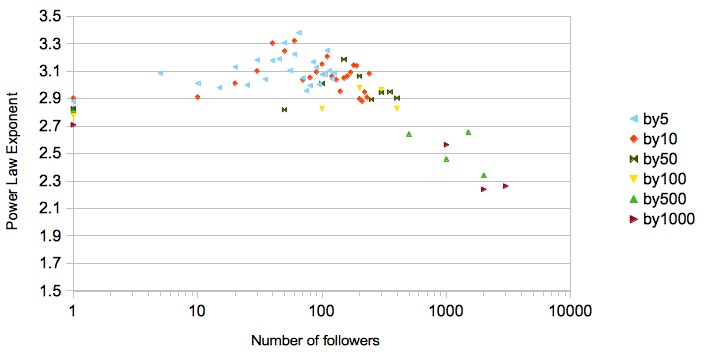
\includegraphics[width=0.5\textwidth]{data/evolutionAlphaParameter.jpg}
\caption{Parameter $\alpha$ of the distribution of retweet chains length according to the number of followers of users}

    \label{fig:evolutionAlphaAll}
\end{figure}

In the following step, we investigated how the parameters of the power law, $\alpha$ and $x_{min}$, are estimated by the follower count of the users.
In Fig. \ref{fig:evolutionAlphaAll} all values of $\alpha$ are plotted. $x_{min}$ do not vary much, being remarkably small, usually between 2 and 3, which means that the power law is valid even to characterize the probability of small chains.
We can observe that the parameter $\alpha$ changes in two phases. Before reaching 100 followers, the value of $\alpha$ is stable or even slightly increasing. But starting from approximately 100 followers and more, the more followers a user have, the higher the value of $\alpha$. This means that the more followers a user have, the higher its probability of being widely retweeted.

We can interpret this result in the following manner: for users with less that 100 followers, this property does not strongly affect the probability of being retweeted. Above 100 followers, more followers means more widely propagated tweets.
From these observations we computed two simple approximations of the relation between $\alpha$ and $FC$. Under a hundred followers the relation is linear, while it is a logarithmic relation above 100. These models are plotted on figures \ref{fig:relationAlphaFVinf} and \ref{fig:relationAlphaFVsup} with their parameters. Though other fitting models could be adopted, we choose these ones for their simplicity.

  \begin{figure}[h]
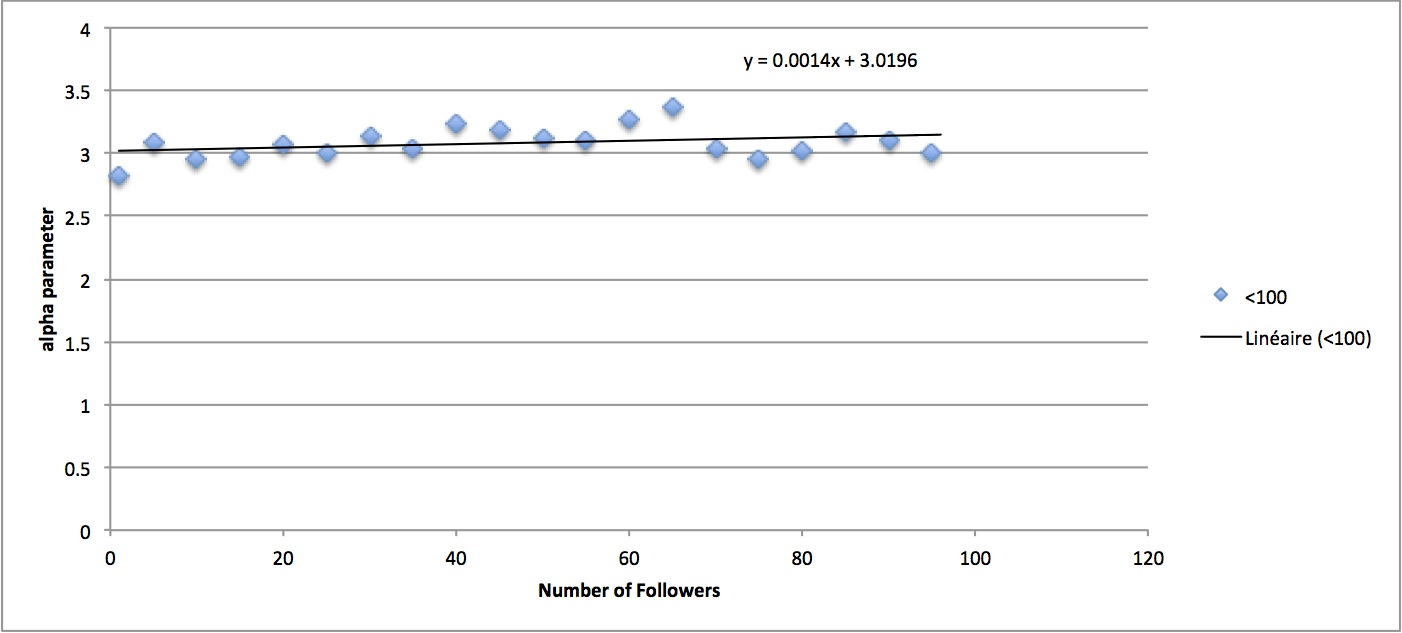
\includegraphics[width=0.5\textwidth]{data/approximationInf100.jpg}
\caption{Relation between $\alpha$ and $FC$ with $FC<100$}

    \label{fig:relationAlphaFVinf}
\end{figure}

  \begin{figure}[h]
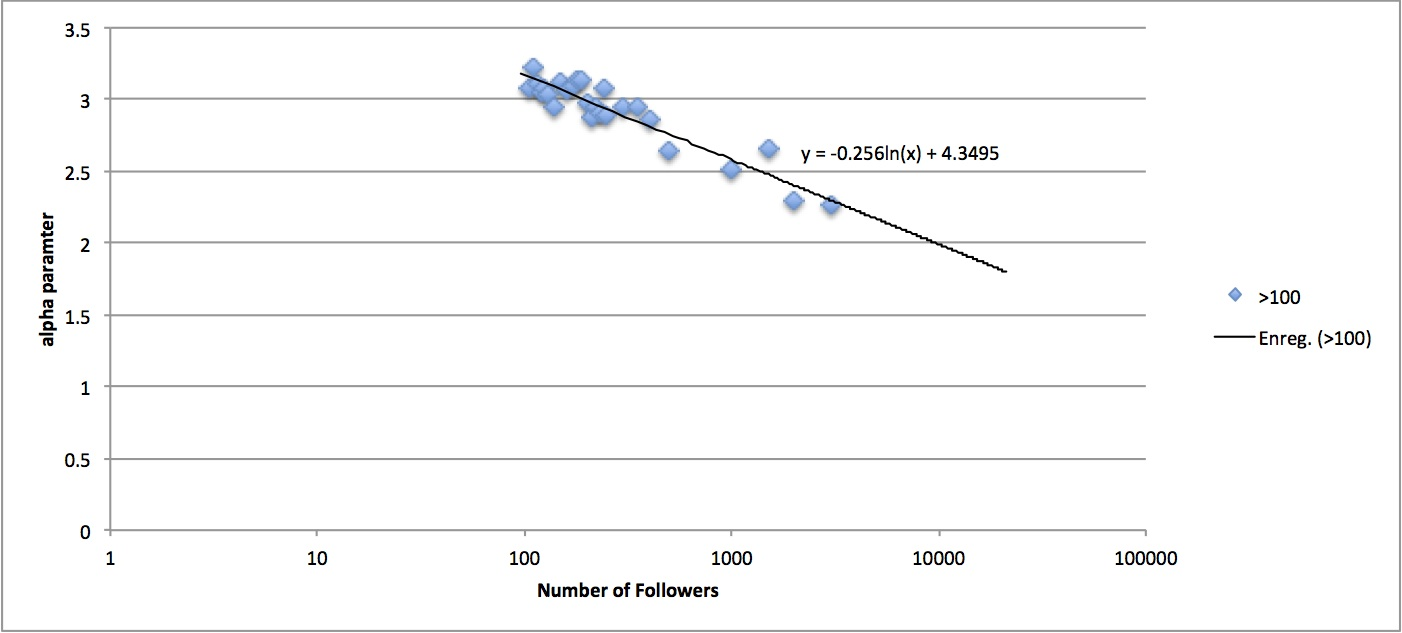
\includegraphics[width=0.5\textwidth]{data/approximationSup100.jpg}
\caption{Relation between $\alpha$ and $FC$ with $FC>100$}

    \label{fig:relationAlphaFVsup}
\end{figure}

\subsection{Validating the model of retweet chain length distribution}

Given a Twitter dataset, we want to propose a simple model that can be used to simulate the propagation of tweets on it without having to consider the content of the tweets or the user-specific behaviors as these properties are highly contextual. Of course, the consequence is that our model will be valid only at the global level and not for the individual users performances. But works such as the one by Bakshy et al.\cite{bakshy2011everyone} have shown that such a precision is not plausible.

Two papers have already proposed models of tweet diffusion. We will begin by presenting these works.
In Yang et al. \cite{yang2010understanding}, the proposed model is based on factor graph model. More precisely, they train their model using 22 features, such as messages' contents, views from followed users, time delay between views of the tweet etc. For each individual tweet posted, the authors attempts to predict the probability of getting retweeted by poster's immediate followers and other followers until the end of the tree. This method is therefore strongly linked to the studied network and to the previous observations. The authors do not give the correspondence of the global properties between the results produced by their model and the observed data.

Another model have been proposed in Yang et al. \cite{yang2010predicting}. The idea is relatively similar: the authors use the Cox proportional hazard regression model to quantify the degree to which a number of features of both users and tweets predict the speed of diffusion. Namely, they use the fact that a tweet uses link or mention, the number of posts of a user, its rate of being mentioned by others, and other parameters which are not specified. Then, they classify tweets in their dataset by topics, and study, for each topic, which factors are the more influential. They found that the important factors vary greatly from topic to topic. As in the previous model, the results obtained are specific to the dataset.

We must also notice a strong possible bias in these models. In both cases, the model is tuned from the data by looking at the retweet chains. These retweet chains are deduced from the content of the tweet. For instance, if a tweet is of the form ``$RT@~u_1:~content$", they will assume that the poster is retweeting the user $u_1$. Similarly, if the tweet is of the form ``$RT@~u_1:~RT@~u_2:~content$", they assume that the tweet was initially posted by $u_2$, and that the current user saw it from $u_1$. However, in reality, this assumption is mostly inaccurate for mainly two reasons:
\begin{itemize}
\item For character limitation reasons, users tend to keep only one user in the ``trace" and therefore, it is not possible to know the real propagation of a tweet from the content of a tweet itself. When using the official retweet option, only the name of the original author of the tweet appears.
\item When a tweet becomes popular, users do not need to follow someone who retweeted it to see it: the tweet can appear on other medias or even as a recommended tweet on Twitter's platform. If users retweet it for this reason, they will only cite the original author.
\end{itemize}
The consequence of these two problems is that we cannot rely on the content of the tweet to study the propagation of tweets. This might, in particular, conduce us to overestimate the impact of the original author in the diffusion.


In the previous section, by studying the data we have observed that the distribution of the length of retweet chain could be represented as a power law, with an $\alpha$ parameter defined as a function of the in-degree of the user. In this section, we show that this model, while being very simple, reproduce accurately the global properties of retweets.


\begin{figure*}[t]
\centerline{\subfloat[Simulated data]{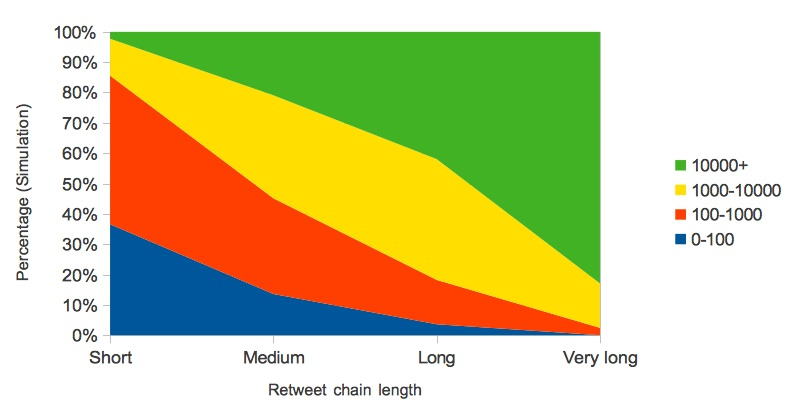
\includegraphics[width=0.5\textwidth]{data/validationProportionsSim.jpg}%
\label{fig_first_case}}
%\hfil
\subfloat[Observations]{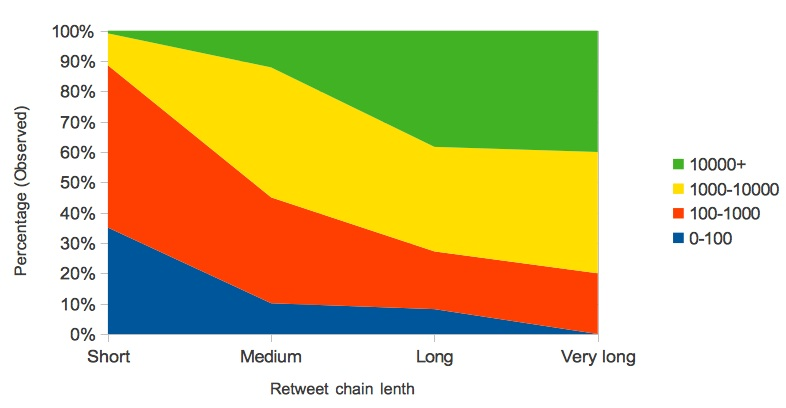
\includegraphics[width=0.5\textwidth]{data/validationProportionsObs.jpg}%
\label{fig_second_case}}}
\caption{Comparison of the proportion of retweets chains of a given length vs. users with a given number of followers. We can observe that our simulation reproduces the properties of the real data, that is, an increasing proportion of tweets made by users with more followers as the length of retweet chains increases.}
\label{fig_sim}
\end{figure*}


In order to do this validation, we adopted the following procedure: for each original tweet published in our dataset on March 10 (the day prior to the earthquake, which was not included in the data used for studying the actual distributions) by a user for whom we know the number of followers, we randomly generate a retweet chain length according to our model. We also count how many times this particular tweet has been actually retweeted. When this operation has been done for all tweets published during this day, we compared the total number of retweets of each length generated by our model to the real numbers. Fig. \ref{fig:evolutionAlpha} shows that the correspondence is very good, which means that, despite the simplicity of the model it fits accurately the data.

However, this result could have been achieved without taking into account the variations in retweetability due to the number of followers. We conducted another test, in which we compare the relative proportions of tweets of a given retweet chain length with given \emph{FC}.

  \begin{figure}[h]
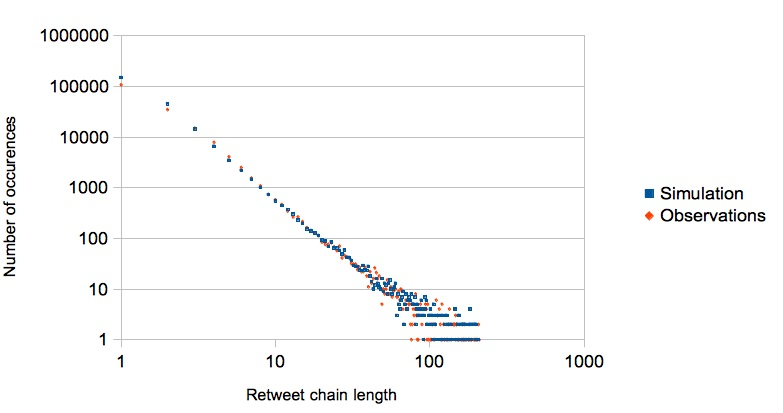
\includegraphics[width=0.5\textwidth]{data/validationModel.jpg}
\caption{Correspondence between retweet chains generated by the model and real retweet chains}

    \label{fig:evolutionAlpha}
\end{figure}

More precisely, we sorted retweet chains in four categories:
\begin{itemize}
	\item Short chains: between 1 and 10 retweets
	\item Medium chains: between 10 and 50 retweets
	\item Long chains: between 50 and 500 retweets
	\item Very long chains: more than 500 retweets
\end{itemize}

We also categorize our users in four:
\begin{itemize}
	\item Few followers: between 0 and 100 followers
	\item Medium number of followers: between 100 and 1000 followers
	\item Many followers: between 1000 and 10000 followers
	\item Super hubs: more than 10000 followers
\end{itemize}

In figure \ref{fig_sim}, we can see that the share of all tweets of a given retweet chain length due to users of a given number of followers follows a very similar pattern in our simulations and in the real network. Interestingly, we see that most short retweets are due to users with few followers. The longer the chains, the higher the proportion of users with a large number of followers. This profile depends on two factors: the difference in probability of having long chains according to the number of followers, and the relative proportion of tweets made by these users. We can however notice that in our simulation, we tend to overestimate the role of users with many followers in very long chains. This might be explained by a cutoff effect on the power law distribution of retweet chain length of these users. As we stated before, the power law model was not perfectly satisfactory for users with very high in-degree, because of a cutoff effect.


\subsection{Effect of the Earthquake}
Several previous works have studied the effect of major crisis on Twitter. Sakaki et al. \cite{sakaki2010earthquake} have shown that such events have an impact so clear on the social network that it is possible to know not only the occurrence of an event such as an earthquake or a typhoon, but also their scale, their precise time of occurrence and location. Earle et al. \cite{earle2010omg} have shown that the increase in the number of tweets during an earthquake has also been used to detect this earthquake. Several other works \cite{mendoza2010twitter} \cite{li2010twitter}  have also used the same phenomenon, the increase in the number of tweets, to capture information about earthquakes.
However, here, we are interested in the effect that such disaster can have on the retweet behavior. We have observed that there are more tweets published during the crisis, but the question arises: is it because there are more unique information published and the retweet behavior is unchanged? or is it because people tend to retweet more?, or a combination of both? By studying the distribution of retweet chains during the period of crisis, we can answer to this question.

 \begin{figure}[h]
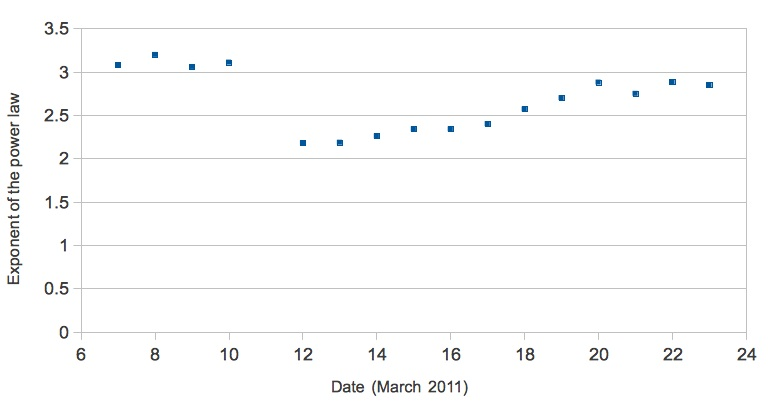
\includegraphics[width=0.5\textwidth]{data/evolutionAlpha.jpg}
\caption{Evolution of the scaling parameter $\alpha$ according to the date. Immediately after the earthquake, the value decreased strongly, which means that a user with the same number of followers before and after the earthquake has a higher probability of being widely retweeted after the earthquake. The value increased slowly in the following days, but cannot reach the pre-event level.}

    \label{fig:evolutionAlphaDate}
\end{figure}

We ran, for each day, the same study on the evolution of the scaling parameter $\alpha$ than we have done for the pre-earthquake period. We found that for each day, the pattern of slow increase until $FC=100$ and then logarithmic decrease was still present. However, we also observed a strong variation of the $\alpha$ values, depending on the day. Figure \ref{fig:evolutionAlphaDate} illustrates this evolution. Each point represents the average value of $\alpha$ for all values of $FC$ in the range 50-100. As we can see, as soon as the earthquake happened, the $\alpha$ parameter decreases strongly. In the following days, this value continuously increase, until coming back to normal values. This mean that for the same user posting the same tweet, the probability of being retweeted is more important after the earthquake than before.
We consequently checked which was the change in behaviors inducing  the more change in the number of tweets published: a raise in retweets or a raise in original tweets. We found that, on the day of the event, the most influential change was the raise in the number of original tweet published, accounting for roughly two thirds of the additional tweets. However, during the following days, the number of original tweets came back to the same levels as before the earthquake, or sometimes even lower. This can be explained by power shortage in some areas after the quake, altogether with a change in behaviors. The percentage of total tweets being retweet, on the contrary, stayed lower than average for several days after the quake, coming back slowly to normal. This comfort our observations. As a conclusion, we can say that, after such a crisis event, there is an important change in the retweet behaviors.

\section{Discussion and usage of the model}
We have seen in the previous section that generating retweet chain lengths according to our observations gives realistic results. Therefore, we can consider using this model to study further the propagation of information on Twitter. When using such a model to study tweet propagation, we always have to keep in mind that our findings are not applicable to any particular tweet. Probably, what will make a tweet successful in the end will be the content of the tweet, the context, and the intrinsic characteristics of the users who publish and see the tweet.

One problem of particular interest for us was the question of the propagation of information in the time of crisis. We know that Twitter has been widely used as a way to propagate information during crisis, in particular when traditional sources of information are not accessible, for catastrophe reasons or even control by another entity. Therefore, one question that we can ask is: how could we ensure the diffusion of an important information to a wide range of users? Or more generally, how users with many followers are better at diffusing information than less popular users? As we said earlier, the particular properties of a tweet are certainly more important than the degree of its poster. However, the impact of this degree on the probability of diffusion of a tweet is not disputable. One could argue that causes and consequences might have been inverted, and that users who publish many popular tweets have many followers because they tend to publish interesting tweets. If that was true, the assumption that the same tweet published by two users with different in-degrees would have different probability of being retweeted would be wrong. However, while it is likely that these users became popular because they tend to publish more interesting tweets than other users, their current status of ``celebrity" actually give them a higher power of propagation due to their large audience. An example of this can be found in \cite{tinati2012identifying}, in which the role of users who are so called amplifier of a tweet is investigated. When these popular users retweet an information published by another less popular user, the further propagation of the tweet is increased strongly. Hence, the same information, tweeted by users of different popularity, achieve different success. It therefore makes sense to study the relative impact of users according to their audience.

\begin{figure}[h]
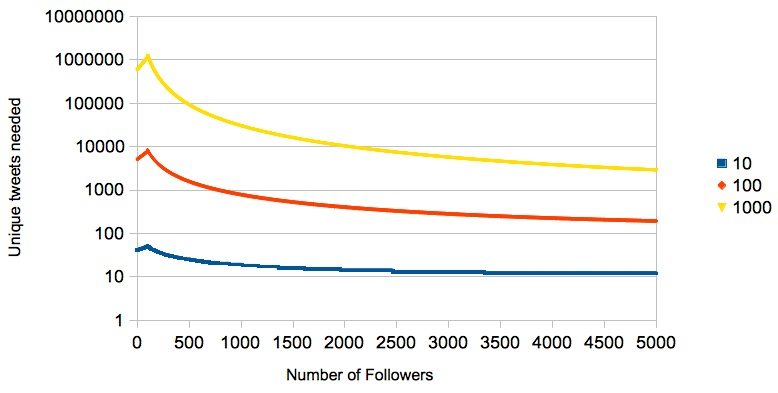
\includegraphics[width=0.5\textwidth]{data/1outOf.jpg}
\caption{Number of unique tweets needed to have one tweet of a given length (10,100 or 1000). The longest the chain, the strongest the difference between popular and less popular users.}

    \label{fig:1outOf}
\end{figure}

The question we want to answer here concerns the probability to publish highly retweeted tweets. For a particular information to reach many people on Twitter, the only possibility is to produce a tweet that is propagated by many. We therefore want to know who are the persons who are the more likely of publishing such information. We know that any user can, of course, publish such a tweet, but we also saw that the probability was much higher for users with more followers. We therefore investigate the probability of producing a tweet of retweet chain length 10, 100 or 1000 according to the degree of the user. We use the parameters of our model described previously to compute one out of how many tweets might reach the objective length. Figure \ref{fig:1outOf} presents the results of this study. We can observe that the difficulty to produce a tweet of a given length vary strongly with the popularity of users. This difference is far more important for long chains than for short chains. When looking at the frequency of tweets of retweet chain length 10, the difference between users of different degree stays always smaller than a factor 10. On the contrary, for tweets of length 1000, the difference between a user followed by 100, and a user followed by 5000 is of a factor more than 100.
This information might be relevant if, for example, one wants to diffuse an information on the network. If the targeted users can be identified, and represent only a small subset of the network, then it is not primordial to have influential users publishing this information. It might be more pertinent to incentive users who belong to this subset, and these users will share it to a short distance in the network, corresponding to the targeted users. On the contrary, if one wants to reach a very broad audience, and think that anyone in the network might have access to this information, then having nodes with a lot of followers publish the information might help, as these users are more likely to generate long chains, that is, to make the information travel further in the network from the original publisher.

These observations are not contrary to the findings presented in \cite{bakshy2011everyone}, but might complete them. In this paper, the authors  investigated roughly the same problem, and came to the conclusion that the impact of users with a lot of followers was not statistically so much greater than users with a few followers. For someone who would like to diffuse a given information on Twitter they therefore recommend to concentrate more on users with few followers, as it is usually easier to make such users diffuse information. However, our results suggest that this is true if we consider the average length of retweet chains. But due to differences in the inclination of the power law ($\alpha$ parameter), this recommendation is to be tempered if one considers that long chains are more important than small ones. One information retweeted one thousand times might give a better diffusion than one hundred pieces of information retweeted only ten times.



% An example of a floating figure using the graphicx package.
% Note that \label must occur AFTER (or within) \caption.
% For figures, \caption should occur after the \includegraphics.
% Note that IEEEtran v1.7 and later has special internal code that
% is designed to preserve the operation of \label within \caption
% even when the captionsoff option is in effect. However, because
% of issues like this, it may be the safest practice to put all your
% \label just after \caption rather than within \caption{}.
%
% Reminder: the "draftcls" or "draftclsnofoot", not "draft", class
% option should be used if it is desired that the figures are to be
% displayed while in draft mode.
%
%\begin{figure}[!t]
%\centering
%\includegraphics[width=2.5in]{myfigure}
% where an .eps filename suffix will be assumed under latex,
% and a .pdf suffix will be assumed for pdflatex; or what has been declared
% via \DeclareGraphicsExtensions.
%\caption{Simulation Results}
%\label{fig_sim}
%\end{figure}

% Note that IEEE typically puts floats only at the top, even when this
% results in a large percentage of a column being occupied by floats.


% An example of a double column floating figure using two subfigures.
% (The subfig.sty package must be loaded for this to work.)
% The subfigure \label commands are set within each subfloat command, the
% \label for the overall figure must come after \caption.
% \hfil must be used as a separator to get equal spacing.
% The subfigure.sty package works much the same way, except \subfigure is
% used instead of \subfloat.
%

%
% Note that often IEEE papers with subfigures do not employ subfigure
% captions (using the optional argument to \subfloat), but instead will
% reference/describe all of them (a), (b), etc., within the main caption.


% An example of a floating table. Note that, for IEEE style tables, the
% \caption command should come BEFORE the table. Table text will default to
% \footnotesize as IEEE normally uses this smaller font for tables.
% The \label must come after \caption as always.
%
%\begin{table}[!t]
%% increase table row spacing, adjust to taste
%\renewcommand{\arraystretch}{1.3}
% if using array.sty, it might be a good idea to tweak the value of
% \extrarowheight as needed to properly center the text within the cells
%\caption{An Example of a Table}
%\label{table_example}
%\centering
%% Some packages, such as MDW tools, offer better commands for making tables
%% than the plain LaTeX2e tabular which is used here.
%\begin{tabular}{|c||c|}
%\hline
%One & Two\\
%\hline
%Three & Four\\
%\hline
%\end{tabular}
%\end{table}


% Note that IEEE does not put floats in the very first column - or typically
% anywhere on the first page for that matter. Also, in-text middle ("here")
% positioning is not used. Most IEEE journals/conferences use top floats
% exclusively. Note that, LaTeX2e, unlike IEEE journals/conferences, places
% footnotes above bottom floats. This can be corrected via the \fnbelowfloat
% command of the stfloats package.



\section{Conclusion and perspectives}
In this paper, we have provided new insights into the propagation of information in Twitter. In particular, we have shown that the distribution of the probability of producing a tweet of a given retweet chain length can be represented as a power law for users of a given in-degree. We have also shown that the parameters of these power laws were different for users of different in-degrees. More notably, we have shown that the parameter $\alpha$ decreases as the number of followers increases with a logarithmic correlation.

Moreover, we have shown that this characterization was pertinent enough to constitute a simple model, allowing us to generate realistic lengths of retweet chains, reproducing some key features of the distribution of long retweet chains. One future work will be to enhance this model by actually generating this retweet chain. On this dataset or another one with the same information, as we know the follower network and the tweets published by all users, we would therefore be able to play alternative versions of the diffusion of information on this network, during a studied period. By comparing the diffusion which actually took place with the generated one, on aspects such as individual information received by each user, or total amount of people informed of a particular piece of information, such as hashtags or URL, we will be able to get more information on how information is diffused on Twitter, on what can be modeled by global properties and what depends on exceptional and unpredictable behaviors or particular users.




% conference papers do not normally have an appendix


% use section* for acknowledgement
\section*{Acknowledgment}
We thank Genta Kaneyama (Cookpad Inc.) for assistance in collecting data from Twitter.





% trigger a \newpage just before the given reference
% number - used to balance the columns on the last page
% adjust value as needed - may need to be readjusted if
% the document is modified later
%\IEEEtriggeratref{8}
% The "triggered" command can be changed if desired:
%\IEEEtriggercmd{\enlargethispage{-5in}}

% references section

% can use a bibliography generated by BibTeX as a .bbl file
% BibTeX documentation can be easily obtained at:
% http://www.ctan.org/tex-archive/biblio/bibtex/contrib/doc/
% The IEEEtran BibTeX style support page is at:
% http://www.michaelshell.org/tex/ieeetran/bibtex/
\bibliographystyle{IEEEtran}
% argument is your BibTeX string definitions and bibliography database(s)
\bibliography{bibliographie.bib}
%
% <OR> manually copy in the resultant .bbl file
% set second argument of \begin to the number of references
% (used to reserve space for the reference number labels box)
%\begin{thebibliography}{1}

%\end{thebibliography}




% that's all folks
\end{document}


